\chapter{Ditt första program}
\begin{multicols}{2}
\section*{\color{MidnightBlue}Du lär dig:}
Skriva kod i en editor.\\
Köra igång ett program.
\section*{\color{MidnightBlue}Uppdrag:}
Skriv detta program i editorn:

\begin{lstlisting}[basicstyle={\ttfamily\fontsize{24}{24}\selectfont}]
sudda
fram
\end{lstlisting}
    
Tryck på den gröna play-knappen\\
för att köra igång ditt program.

\columnbreak

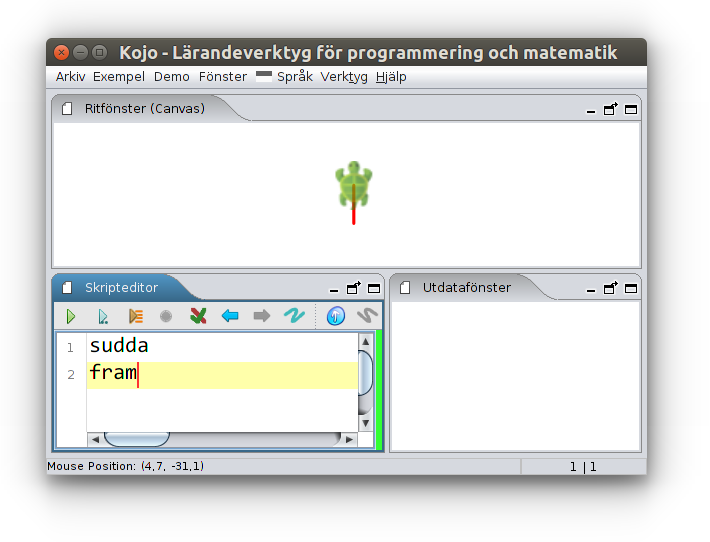
\includegraphics[width=14cm]{../img/fram.png}
\end{multicols}

